% Chapter 1

\chapter{Introduction} % Main chapter title

\label{ch:intro} % For referencing the chapter elsewhere, use \ref{Chapter1} 

%----------------------------------------------------------------------------------------

% Define some commands to keep the formatting separated from the content 
\newcommand{\keyword}[1]{\textbf{#1}}
\newcommand{\tabhead}[1]{\textbf{#1}}
\newcommand{\code}[1]{\texttt{#1}}
\newcommand{\file}[1]{\texttt{\bfseries#1}}
\newcommand{\option}[1]{\texttt{\itshape#1}}
\newcommand{\enquote}[1]{``#1"}
%----------------------------------------------------------------------------------------

In 1965 at Bell Labs, Arno Penzias and Robert Wilson serendipitously detected "noise" with their microwave antenna.  This noise was isotropic (same in all directions) and homogenous (same in all locations), and was ultimately the measurement of the cosmic microwave background; radiation from the early universe.
\begin{equation}
    I(\nu,T) = \frac{2h\nu^2}{c^2}\frac{1}{e^{\frac{h\nu}{k_B T}} -1}
    \label{eq:blackbody}
\end{equation}
The temperature power spectrum of the CMB was measured to be a near-perfect black-body (Eq.~\ref{eq:blackbody}), with a mean temperature of~\cite{burke_graham-smith_wilkinson_2019}:
\begin{equation}
    T_{\text{CMB}} = 2.725\,K
\end{equation}
The power spectrum lies in the infra-red range of the electromagnetic spectrum, and peaks at a wavelength $\lambda = 1.5\,\text{mm}$ (Figure~\ref{fig:cobe_power_spectra}). 

This near-perfect black-body is understood to originate during the early universe by the rapid collision of photons with free electrons, to keep radiation in thermal equilibrium with hot dense matter.  As the universe expanded and cooled, however, this spectrum has kept its same form~\cite{weinberg_cosmo}.  Because it formed during the early universe, the CMB is a backlight into not only early universe properties, but also late universe physics such as large-scale structure and dark matter.  The CMB, therefore, carries a wealth of information about the fundamental physics of our universe.

\begin{figure}[t]
    \centering
    \includegraphics[width = .95\textwidth]{Figures/cobe_power_spec.pdf}
    \caption{Right: Spectrum of the CMB from the COBE satellite~\cite{1994ApJ...420..439M}.  The deviation from an ideal blackbody is magnified $\times\,400$ in the bottom panel.  Left: First-year maps from the COBE Differential Microwave Radiometer in 1992~\cite{1992ApJ...396L...1S}.}
    \label{fig:cobe_power_spectra}
\end{figure}

\section{The Expanding Universe}
The evolution of the universe can be described with an extension of Einstein's equations.  To measure distances in an expanding universe, we employ the metric $ds$, which depends on the curvature of the surface:
\begin{equation}
    ds^2 = -c^2dt^2 + a(t)^2[dr^2 + S_\kappa (r^2)d\Omega^2]
\end{equation}
where
\begin{equation}
    d\Omega^2\equiv d\theta^2 + \sin^2\theta d\phi^2
\end{equation}
and
\begin{equation}
    S_\kappa(r) = \begin{cases} R\sin(r/R) & (\kappa = +1) \\
  r & (\kappa = 0) \\
   R\sinh(r/R) & (\kappa = -1)\end{cases}
\end{equation}
Here we consider the scale of the universe as a function of time $a(t)$, which relates to the redshift $z$ as:
\begin{equation}
    a(t) = \frac{1}{a+z}
\end{equation}
where we set today's $a=1$.  If $a(t)$ is increasing, then the object is "red-shifted", or a decrease in frequency.  This relationship can be expanded for nearby sources:
\begin{equation}
    a(t)\approx a(t_0)[1+(t-t_0)H_0+ \ldots ]
\end{equation}
where we've introduced the Hubble Constant $H_0$.  The Hubble Constant quantifies the expansion of our universe:
\begin{equation}
    H_0\equiv \bigg(\frac{\dot{a}}{a}\bigg )_{t=t_0}
\end{equation}

\section{The Three Equations of the Universe}

The dynamics of the universe are neatly described by three equations, which connect its curvature to the energy density $\epsilon$ and pressure $P$.

\noindent
\textbf{Friedmann Equation}:  Stemming from Einstein's relativistic field equations, the Friedmann equation describes a homogenous and isotropic universe:  
\begin{equation}
    \bigg ( \frac{\Dot{a}}{a} \bigg ) = \frac{8\pi G}{3c^2}\epsilon(t) - \frac{\kappa c^2}{R_0}\frac{1}{a(t)}
\end{equation}
where $\epsilon$ is the energy density, $G$ is the gravitational constant, $c$ is the speed of light, $\kappa$ is the curvature parameter, and $R_0$ is the radius of curvature at present time $t=0$.  The energy density is evolving, and made up of matter ($\epsilon_m=\epsilon_{m0}a^{-3}$), radiation ($\epsilon_r=\epsilon_{r0}a^{-4}$), and a cosmological constant ($\epsilon_{\Lambda}=\epsilon_{\Lambda 0}$), thus the Friedman equation takes the form:
\begin{equation}
    \frac{H^2}{H_0^2} = \frac{\Omega_{r0}}{a^4} + \frac{\Omega_{m0}}{a^3} + \Omega_{\Lambda 0} + \frac{1-\Omega_0}{a^2}
\end{equation}
where we normalize the energy density $\epsilon$ by the critical density $\epsilon_c(t)$, where $\epsilon_c(t) = \frac{3c^2}{8\pi G}$~\cite{ryden_2016}.  This results in the new variable:
\begin{equation}
    \Omega(t) = \frac{\epsilon(t)}{\epsilon_c(t)}
\end{equation}
The $\Lambda$CDM model assumes a flat $\Omega(t)=1$ universe, comprised of baryonic $\Omega_b h^2$ and cold dark matter $\Omega_c h^2$ densities.
\noindent
\textbf{Fluid Equation}:  Energy conservation can also be applied to describe the dynamics of the universe via the first law of thermodynamics (Eq.~\ref{eq:thermo1}).  This implies the sum of gravitational potential and kinetic energy of expansion is conserved~\cite{ryden_2016}.
\begin{equation}
    dQ = dE + PdV
    \label{eq:thermo1}
\end{equation}
\begin{equation}
    \dot{\epsilon} + \frac{3\dot{a}}{a}(\epsilon + P) = 0
    \label{eq:fluid_universe}
\end{equation}
\noindent
Solving the fluid equation (with $P=w\epsilon$) yields the equation of state:
\begin{equation}
    \epsilon \propto a^{-3-3w}
\end{equation}
with the time-independent $w$~\cite{weinberg_cosmo}.  For example, in the case of cold matter dominated universe (e.g. dust, $P = 0$) $\epsilon\propto a^{-3}$, and in a hot matter universe (e.g. radiation, $P=\epsilon/3$) $\epsilon\propto a^{-4}$.
\noindent
\textbf{Acceleration Equation}: Combining the first two equations, which constrain an energy conserved universe, yields the acceleration equation describing how our universe expands over time.  
\begin{equation}
    \frac{\ddot{a}}{a} = - \frac{4\pi G}{3 c^2} (\epsilon + 3 P)
\end{equation}
\section{The CMB Temperature Power Spectra}
The cosmic microwave background carries rich science in its temperature and polarization spectra.  The CMB power spectra can be decomposed into spherical harmonics, which result in power spectra as a function of multipole moment $\ell$, where $\ell\approx180/\theta$.  The temperature fluctuations of the CMB are decomposed into spherical harmonics:
\begin{equation}
\frac{\delta T}{T}(\theta,\phi) = \sum_{\ell=2}^{\infty} \sum_{m=-\ell}^{\ell} a_{\ell m} Y_{\ell m}(\theta,\phi)
    \label{eq:cmb_temp}
\end{equation}
where $\ell$ and $m$ are multipoles of the spherical harmonic $Y_{\ell m}$, $a_{\ell m}$ are expansion coefficients, and $\theta$ and $\phi$ represent the angular position on the sky.  The coefficients $a_{\ell m}$ are independent variables, and relate to the CMB's angular power spectra via:
\begin{equation}
    C_\ell^{TT} = \frac{1}{2\ell +1} \sum_{m=-\ell}^{m=\ell} |a_{\ell m}|^2
\end{equation}
This is the temperature power spectrum of the CMB.  Figure~\ref{fig:measured_cmb_spec} shows the measured CMB temperature power spectrum from the Atacama Cosmology Telescope, the South Pole Telescope, and WMAP~\cite{Das_2014}.
\begin{figure}[t]
    \centering
    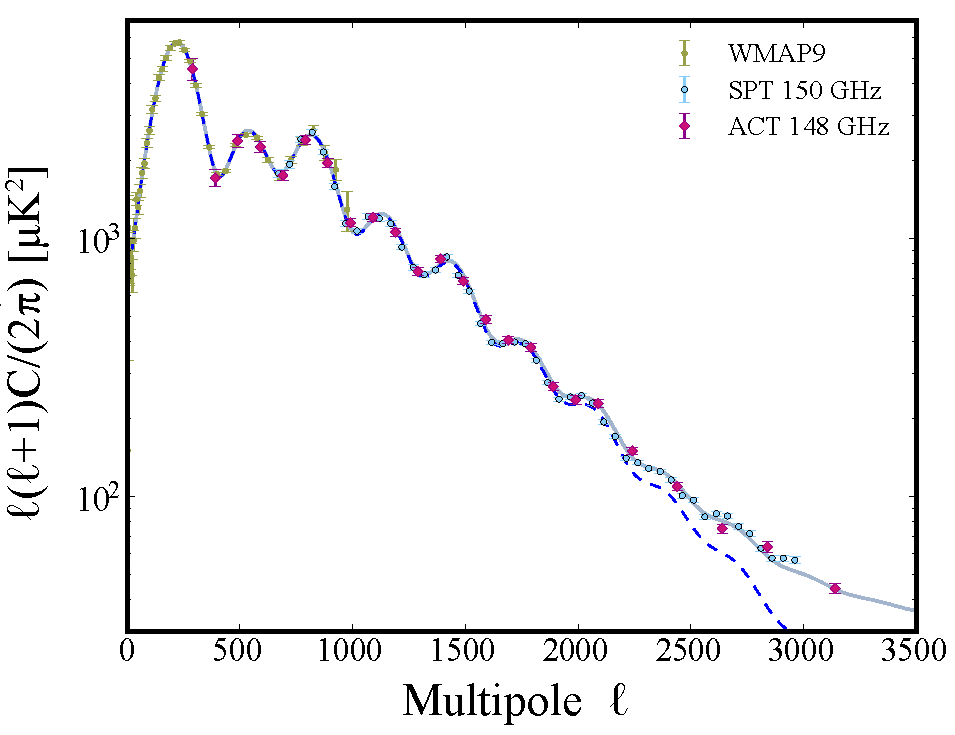
\includegraphics[width = .75\textwidth]{Figures/temp_power_spectrum.pdf}
    \caption{The CMB temperature power spectra measured by WMAP (yellow), the South Pole Telescope (blue) and the Atacama Cosmology Telescope (purple)~\cite{Das_2014}.  The temperature anisotropies of the CMB will be measured with the Simons Observatory and CMB-S4, two upcoming cosmology experiments, with further precision.}
    \label{fig:measured_cmb_spec}
\end{figure}
The shape of the CMB power spectra unlocks properties of the early universe.  For example, the first peak in the power spectrum at around $\ell\approx220$ corresponds to the angle at which we observe the sound horizon, or the distance that sound can travel between the big bang and recombination.  The measurement of this power spectrum's morphology can also determine physical matter ang baryon densities.  The dark energy properties of our universe can additionally be constrained by the power spectrum peak, as the dark energy and matter densities jointly alter the distance to last scattering.  The smaller angular scale distortions are in part due to an inhomogeneous universe at the time of last scattering ($z\approx 1100$). 

\section{The Polarized CMB}
The cosmic microwave background is predicted to be polarized, due to Compton scattering by free electrons during the era of recombination~\cite{}.  Measuring this polarization would indicate the beginning of reionization and further have the potential to uncover effects of primordial gravitational waves.  The electric field of a photon travelling in the $\hat{z}$-direction is described by:
\begin{figure}
    \centering
    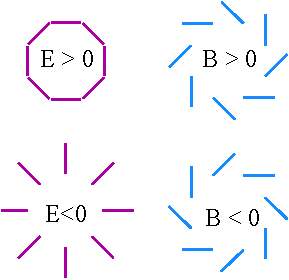
\includegraphics[width = .45\textwidth]{Figures/EB_pol.pdf}
    \caption{The polarization modes of the CMB.  The E modes have no curl, while the B modes have no divergence.  The polarization pattern in the CMB is caused by...}
    \label{fig:e_b_pol}
\end{figure}
\begin{equation}
    \Vec{E} = (E_x\hat{x} + E_y\hat{y})e^{i k_z - \omega t }
\end{equation}
We measure the polarization signal of the CMB with Stokes parameters, which we obtain from the electric field $\Vec{E}$, with intensity $I$, linear polarization $Q$, diagonal polarization $U$, and circular polarization $V$ (Eq.~\ref{eq:stokes}).
\begin{equation}
\begin{split}
    I & = |E_x|^2 + |E_y|^2 \\
    Q & = |E_x|^2 - |E_y|^2 \\
    U & = E_x E_y^* + E_x^*E_y\\
    V & = i(E_x E_y^* - E_x^*E_y) \\
\end{split}
\label{eq:stokes}
\end{equation}
Just as the temperature power spectrum is decomposed into spherical harmonics, we express the polarization of the CMB in terms of spin-2 (where $a^*_{-2,\ell m} = a_{2,\ell m}$) spherical harmonics:
\begin{equation}
(Q \pm iU) = \sum_{\ell m}^{\pm 2} a^{\pm 2}_{\ell ,m} Y_{\pm2,\ell m}
\end{equation}
\begin{equation}
\begin{split}
    a_{\ell m }^E & = -\frac{1}{2}(a_{\ell m}^2 + a_{\ell m}^{-2}) \\
    a_{\ell m }^B & = \frac{i}{2}(a_{\ell m}^2 - a_{\ell m}^{-2})
\end{split}
\end{equation}
The E- and B-modes of the CMB are defined as:
\begin{equation}
\begin{split}
    E(\theta,\phi) & = \sum_{\ell m} a_{\ell m }^E Y_{\ell m}(\theta,\phi) \\
    B(\theta,\phi) & = \sum_{\ell m} a_{\ell m }^B Y_{\ell m}(\theta,\phi)
\end{split}
\end{equation}

\section{Status of the Field}
Since the detection by Penzias and Wilson in 1965, the cosmology community has made leaps to constrain the black-body of the CMB.  

\begin{table}[t]
    \centering
    \begin{tabular}{|c|c|c|}\hline 
         Parameter & Planck 20XX Release & ACT 20XX Release \\
         $\Omega_b h^2$ &  & \\
         $\Omega_c h^2$ &  & \\
         $n_s$ &  & \\
         $\tau$ &  & \\ \hline
    \end{tabular}
    \caption{The most recent cosmological parameters as from the 20XX Planck release[YYY] and the 20XX ACT release~[XXX].}
    \label{tab:cosmology_recent_results}
\end{table}

The Cosmic Background Explorer (COBE) was the first to measure the CMB power spectrum from space.  Since COBE, the measurement of the black-body of the CMB has increased in precision, with experiments like WMAP, Planck, for example.  The South Pole Telescope and the Atacama Cosmology Telescope, two ground-based telescopes, have pushed the measurement further with increased resolution mapping of the sky.

Now going for polarization signal...

Who has detected the lensed B-mode. 

% \section{Atacama Cosmology Telescope}

% \begin{figure}
%     \centering
%     \includegraphics[width = .8\textwidth]{Figures/act_perspective2.jpeg}
%     \caption{The Atacama Cosmology Telescope site.  The outer ground screen protects the telescope from stray light.  The inner co-moving ground-screen further protects the telescope from stray light during ovservations.}
%     \label{fig:act_site}
% \end{figure}
% \subsection{Science Goals}
% \subsection{Instrument Overview}

% \begin{figure}[t]
%     \centering
%     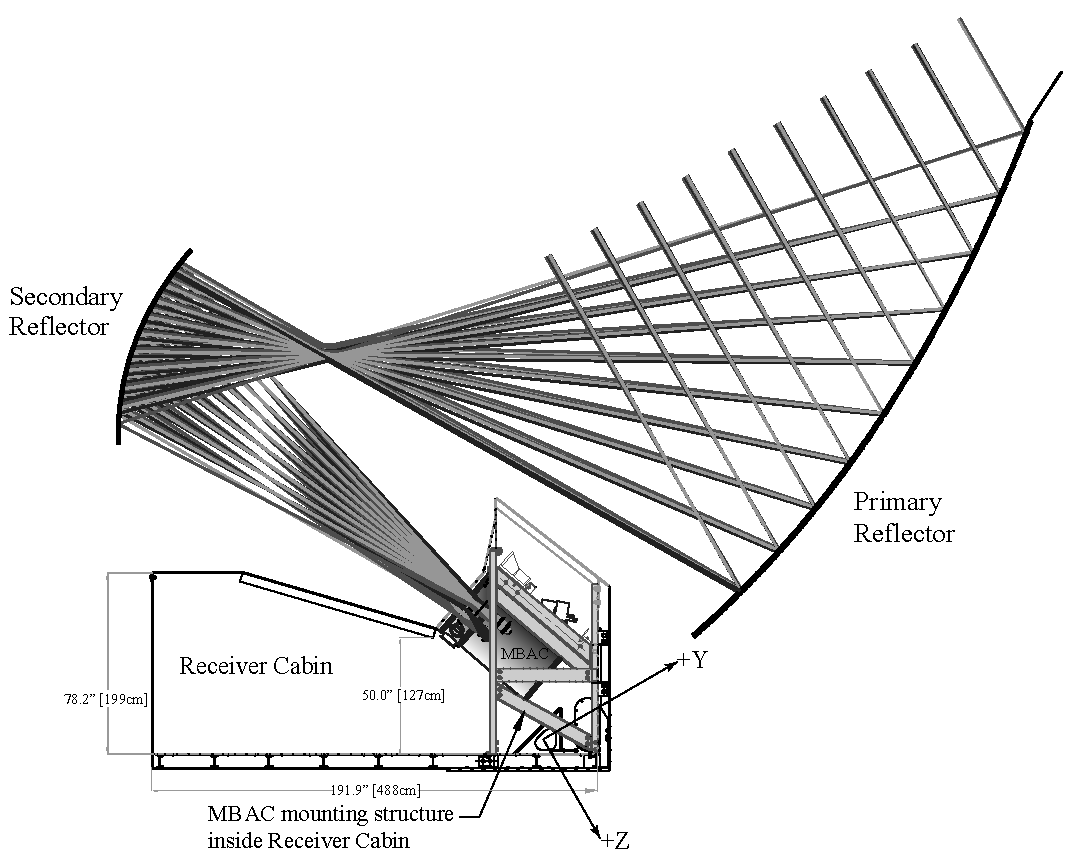
\includegraphics[width = .8\textwidth]{Figures/act_inst.pdf}
%     \caption{Ray-trace diagram of the Atacama Cosmology Telescope~\cite{act_inst}.  The telescope is an off-axis Gregorian with two reflectors: the primary is 6\,m in diameter and the seconday 2\,m.  The rays trace into the Millimeter Bolometer Array Camera (MBAC) cryostat which houses the telescope's detectors.}
%     \label{fig:act_inst}
% \end{figure}

% \begin{table}[t]
%     \centering
%     \begin{tabular}{|l|l|l|l|} \hline
%         \textbf{ Parameter} &  \textbf{PA4 F150} &  \textbf{PA5 F090}  &  \textbf{PA6 F090}  \\ \hline \hline
%         Number of Bolometers & 510 & 510 & 510\\\hline
%         Center Frequency (GHz) & 150\,GHz & 90\,GHz & 90\,GHz\\\hline
%         Base Temperature & 100\,mK & 100\,mK & 100\,mK\\\hline
%         % Angular Resolution & 1 arcmin &1 arcmin &1 arcmin\\\hline
%         % Solid Angle & & &\\\hline
%         % Sky Coverage & & &\\\hline
%     \end{tabular} \caption{ACT Key Characteristics.}
%     \label{tab:act}
% \end{table}

% \section{The Simons Observatory}

% \begin{figure}[t]
%     \centering
%     \includegraphics[width=\textwidth]{Figures/Site_Drone_Picture_July_2019.jpeg}
%     \caption{The Simons Observatory and Atacama Cosmology site in the Atacama Desert, Chile.}
%     \label{fig:act_so_site}
% \end{figure}
% \subsection{Science Goals}

% SO will test cosmic inflation during the early universe, characterize the primordial perturbations, measure the effective number of relativistic species and the sum of the neutrino masses, and improve our understanding of galaxy evolution and the era of cosmic reionization~\citep{so19}. 

% \subsection{Instrument Overview}

% \begin{figure}[t]
%     \centering
%     \includegraphics[width = .8\textwidth]{example-image-a}
%     \caption{Ray-trace diagram of the Simons Observatory Large Aperture Telescope~\cite{XX}.  The telescope is a cross-Dragone with two reflectors, both 6\,m in diameter.  The rays trace into the Large Apertue Telescope Receiver (LATR) cryostat which houses 13 optics tubes.  The optics tubes guide the photons onto the detectors in the focal plane, which are cooled to 100\,mK.}
%     \label{fig:act_inst}
% \end{figure}

% The Simons Observatory (SO) is a series of millimeter-wave telescopes designed to observe the Cosmic Microwave Background (CMB) temperature and polarization signals to an unprecedented sensitivity~\cite{gali18, so19}. With the combination of one Large Aperture Telescope (LAT)~\cite{xu/etal:2020c, zhu18, orlo18, coppi/etal:2018} and three Small Aperture Telescopes (SAT)~\cite{ali20}, the experiment will measure the temperature and polarization anisotropy of the cosmic microwave background with $\sim$\,70,000 background noise limited detectors operating at $\sim$\,100\,mK. 

% The Simons Observatory was deployed in the Parque Astronomico located in the Atacama Desert in Chile. The telescope site is situated at an elevation of 5200 meters near the peak of Cerro Toco at $22 ^\circ$ 57' S, $67^\circ$47' W. The arid conditions and elevation at the site minimize contamination to millimeter wave signals from water vapor. 

% \begin{table}[t]
%     \centering
%     \begin{tabular}{|l|l|l|l|} \hline
%         \textbf{ Parameter} &  \textbf{LF} &  \textbf{MF}  &  \textbf{UHF}  \\ \hline \hline
%         Number of Bolometers & $>$20,000& $>$20,000& $>$20,000\\\hline
%         Base Temperature & 100\,mK & 100\,mK & 100\,mK\\\hline
%         Angular Resolution & 1 arcmin &1 arcmin &1 arcmin\\\hline
%         Solid Angle & & &\\\hline
%         Center Frequency (GHz) & 27-270\,GHz & 27-270\,GHz & 27-270\,GHz\\\hline
%         Sky Coverage & & &\\\hline
%         Sensitivity & & &\\\hline
%         % Detector Time Constants & & & \\\hline
%         % Polarization Modulation & & &\\\hline
%         Location & Ground (Chile)& Ground (Chile)& Ground (Chile)\\
%         \hline
%     \end{tabular} \caption{SO Key Characteristics.}
%     \label{tab:so}
% \end{table}

% \subsection{Optics}
% The primary mirror is 6 m in diameter and constructed out of 77 individual adjustable panels, while the secondary mirror is 6 m in diameter and constructed out of 69 adjustable panels \cite{gali18}.

\section{Outline of Thesis}

First, I overview two ground-based cosmology experiments in Chapter~\ref{ch:instruments}: the Atacama Cosmology Telescope (ACT) and the Simons Observatory (SO).  This work focuses on the development and characterization of optical components for the Simons Observatory.  In the final chapter of this work, I characterize the optical performance of ACT.

In Chapter~\ref{ch:mma}, I present an overview of the meta-material absorbers used in the Simons Observatory Large Aperture Telescope optics tubes to control stray light.  I also present the characterization of their optical properties using a radio holography receiver.  These tiles are comprised of an outer metamaterial layer, which approximates a lossy gradient index anti-reflection coating. They are fabricated via injection molding commercially-available carbon-loaded polyurethane (25\% by mass). The injection molding technology enables mass production at low cost.  Room temperature optical measurements verify their control of reflectance to less than 1\% up to 65$^{\circ}$ angles of incidence, and control of wide angle scattering below 0.01\%.

The characterization of optical components is continued in Chapter~\ref{ch:si}, where I characterize the reflectivity and loss tangent measured in the W-band (80-125\,GHz) and D-band (125-180\,GHz) in two samples of float zone silicon with intrinsic stoichiometry - one irradiated by neutrons, which increases the resistivity by introducing crystalline defects, and the other unperturbed.  I find the loss tangent $\tan\delta$ of $2.8\times10^{-4}$ and $1.5\times10^{-5}$ for neutron-irradiated silicon and intrinsic silicon, respectively, both with an index of refraction of 3.41.  The results demonstrate the applicability of silicon as a warm optical component in millimeter-wave receivers.  The depth of the reflection nulls provides a sensitive measurement of dielectric losses.

In Chapter~\ref{ch:ot_holo}, I present near-field radio holography measurements of the SO LATR optics.  These measurements demonstrate that radio holography of complex millimeter-wave optical systems comprising cryogenic lenses, filters, and feed horns can provide detailed characterization of wave propagation before deployment.  I used the measured amplitude and phase, at 4\,K, of the receiver near-field beam pattern to predict two key performance parameters: 1) the amount of scattered light that will spill past the telescope to 300\,K and 2) the beam pattern expected from the receiver when fielded on the telescope.  These cryogenic measurements informed the removal of a filter, which led to improved optical efficiency and reduced side-lobes at the exit of the receiver.  This is the first time such parameters have been confirmed in the lab prior to deployment of a new receiver.

Chapter~\ref{ch:holosim} presents Holosim-ML: a Python code for beam simulation and analysis of radio holography data from complex optical systems.  This code uses machine learning to efficiently determine the position of hundreds of mirror adjusters on multiple mirrors with few micrometer accuracy.  I apply this approach to the example of the Simons Observatory 6\,m telescope.

Exploring Atacama Cosmology Telescope beams in Chapter~\ref{ch:actbeams}, 

% Lastly, in Chapter~\ref{ch:conclusion}, 